%\todo[inline]{existing game research?? own section?}

\section{Games and the Virtual Reality}
\label{sec:gamesNvr}

To catch a brief insight into games that both support playing with or without HMD and to further introduce research aspects of the following section this paragraph is intended to list a few differences, similarities and uniqueness within games. An overview of these games can be found in Table~\ref{tab:popularGames}, where some properties of them are listed. 

Starting with \textit{Minecraft}~\cite{game:minecraft}. an open world sandbox game where the player controls his playable character by navigating with the keyboard or game controller. The goal is to mine blocks of different material and craft them into objects which he will need to complete the game. As it is an open world game the player can move to different areas in order to gather some items needed~\cite{game:minecraft}. \newline
A disadvantage of this game in VR is the locomotion method needed in order to move around the world. Since the game has not many stationary tasks and it depends on the ability of the user to move around it holds greater potential for the virtual reality sickness (Explanation see Section \textit{Further Research Trends: Increasing The Performance Of Devices For VR Gaming}) occurring.

Another game is \textit{Keep Talking and Nobody Explodes}~\cite{game:keepTalking} a puzzle game where one player has to describe and disarm a virtual explosive charge in a given time. His team members, who cannot see the bomb, have to explain what he has to do in order to disarm the bomb and to save his and the team members lives~\cite{game:keepTalking}. The game mechanics are different from those of Minecraft. The player wearing the HMD has a stationary task and just needs to interact with objects in his direct vicinity. \newline
Because of this only natural locomotion the peril of becoming sick is very weakly present.

\begin{figure}
	\centering
	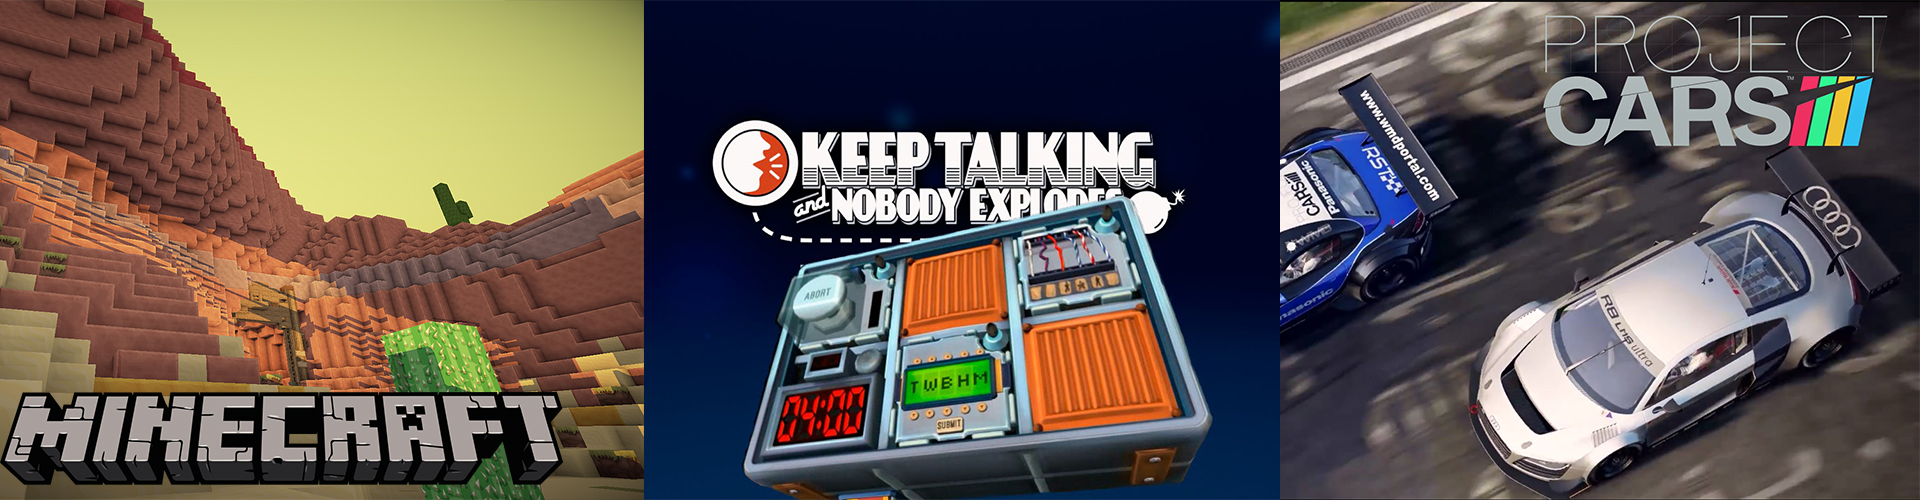
\includegraphics[width=0.99\columnwidth]{./figures/banner}
	\caption[banner]{The three presented games. FLTR Minecraft, Keep talking and nobody explodes and Project CARS. Each game offers native VR Support on multiple devices and has different interaction methods for locomotion. Image source in footnote 1 \textcolor{white}{\footnotemark[1]}}~\label{fig:banner}
\end{figure}
\footnotetext[1]{
	\textcopyright~Mohjang, Steel Crate Games, Slightly Mad Studios, [Online; accessed January 04., 2017],[Digitally edited] \url{https://pixabay.com/p-354458} \url{https://i.ytimg.com/vi/Apwa_ksMvM0/maxresdefault.jpg} \url{https://i.ytimg.com/vi/RggvBJ2ANWo/maxresdefault.jpg} \ccbyncsa
} 
\textit{Project CARS} is a racing simulation for Microsoft Windows, PlayStation 4, and Xbox One~\cite{game:projectC}. It offers standard racing simulation whilst offering HMD based gameplay as well as normal gameplay using a monitor. The game depends on content created by its users to extend the gaming experience~\cite{game:projectC}. \newline
The locomotion is solely a cockpit locomotion, meaning that the player is sitting in a virtual car and steering with different interfaces. Because of the visual stimuli of moving inside a car but neither the vibration nor the acceleration is palpable the user could be more weakly prone to becoming VR sick.

In VR these games offer an immersive way to include the gamer into the game. Because of the different approaches to solving problems of VR more static games like \textit{Keep Talking and Nobody Explodes} and \textit{Project CARS} could have greater potential in becoming very popular in the VR gaming community. 

%There are no numbers available regarding the players per month that are using 
%VR for their gaming experience in these games. 

%\blindtext[1]

\begin{table}%[h]
	\caption{Popular games played in late 2016. The games offer a regular play mode, using the monitor, and a VR play mode with both the Oculus Rift and the HTC Vive. Types of Locomotion (LM): Natural Locomotion (NLM), Cockpit Locomotion (CLM), Artificial Locomotion (ALM). RPG: Role-Playing Game}~\label{tab:popularGames}
	
	%{}\fontfamily{pcr}\selectfont
	\renewcommand{\arraystretch}{1.3}% for the vertical padding
%	\small
	\begin{tabular*}{\columnwidth}{ p{33mm} l r l }
		Gametitle & Genre & \parbox[c][2.2em][t]{2cm}{\begin{flushright}$\dfrac{Players}{Month}$(\footnotemark[2])\end{flushright}} & LM \\
		\hline
		Minecraft & RPG & 990 K & ALM \\
		Keep Talking and \newline Nobody Explodes & Puzzle & 153.3 & NLM \\
		Project CARS & Racing & 1.01 K & CLM\\
	\end{tabular*}
	%}
	
\end{table}

\footnotetext[2]{\url{http://steamcharts.com}, accessed Jan. 3., 2017}
%\todo[inline]{Die footnotes werden nicht richtig nummeriert... von hand fixen bei submission!?}

\subsection{Popularity Of VR Games}
Since the beginning of game development and virtual reality in the 20th century there has been a huge potential to include the user in a virtual environment. Some systems have been developed in the past five years that simplify some processes of work for different disciplines. 

Games have just lately adopted the potential for this immersive form of gaming. VR offers new dimensions of freedom to include the player into a game world and to tell stunning stories.

Using a virtual environment to show worlds to players has the great advantage of giving them the feeling of being in the middle of the event, but the game has very limited possibilities to tell stories with much variety. This is that the game can not change perspectives as easy. 

While games that do not use VR can handle attention themselves by just moving the camera, VR is bound to the camera perspective of the gamer. These games can show views from other perspectives without worrying about the user becoming confused. VR games need another way to handle interactiveness, the user has to hold some kind of controller interface to tell the system what he wants to do. Games outside of VR have similar interface problems but the process has been researched more than the interaction with VR games. Simultaneously VR games require a much more active way of interaction, because the user has to complete physical tasks as he is playing the game. This can be a negative point for people who would just rather enjoy a game than have a minor workout while playing.

It is not yet set whether the implementation of VR into the three games from above has increased the popularity drastically. Official values regarding players and other statistics are hard to acquire. Certainly the game developers have not had losses in terms of player count after implementing VR support since the games are popular for regular players already. \newline
Virtual reality offers a broad new way of experiencing games. Why is it that the virtual reality has not yet reached a higher popularity with a wide range of players?

\divider

In January 2017 I have created an online survey asking players and non players alike on their opinion regarding virtual reality and games. Withing the 5 days of activity of the survey almost 50 participants had taken part in it. Although I have only scratched the surface of the topic with this number of participants a very good overview of different gaming generations can be given. The age spanned from 12 to 50 years.\newline
The survey showed that a majority of people had never played a virtual reality game before. When asked why the most common answer was regarding the pricing of VR systems in general. Some people answered that they did not have enough space in their living room and others said they where not satisfied with the quality and development of VR as of today. This opens up another question that researchers have to tackle: is VR gaming a luxury good reserved for only a few? \newline
It was further found that most persons describing themselves as gamers would agree that VR games should be immersive and intuitive. The results can be seen in Table \ref{tab:study} as well as Figure \ref*{fig:study}. Intuitive meaning that the interaction and locomotion in the game is as close as possible to movement in the real world. Most participants agreed that VR do not have to be simple regarding interaction and problems presented. \newline 
The study has lastly shown that most of the people that have tried a VR game in person would describe themselves as gamers, although also many other participants affirmed this question.\newline The last question resulting is if people are more likely to test VR in person if they think they already are gamers or if VR games can reach a broader audience in the future due to the higher approachability of games. Every person knows how to pull a virtual bow since it is close to real world interaction rather than interacting with other interfaces. 

\begin{table}[h]
	\caption{Gamers and non games have been asked to rate the following aspects, whereas 1 means they strongly disagree, 4 means they strongly agree - 0: unsure. The question asked was whether they thing a VR game should be...}~\label{tab:study}
	
	\renewcommand{\arraystretch}{1.3}% for the vertical padding
%	\small
%	\rowcolors{2}{gray!15}{white}
	\begin{tabular*}{0.98\columnwidth}{ p{28mm} | @{\extracolsep{\stretch{1}}}*{5}{r}@{}}
		 & 1 & 2 & 3 & 4 & 0 \\
		\hline
		Immersive & 0 & 0 & 10 & 37 & 2 \\
		Active & 2 & 11 & 23 & 11 & 2 \\
		Intuitive & 0 & 2 & 24 & 19 & 4 \\
		Simple & 5 & 25 & 10 & 4 & 5 \\
	\end{tabular*}
	
\end{table}

\begin{figure}[h]
	\centering
	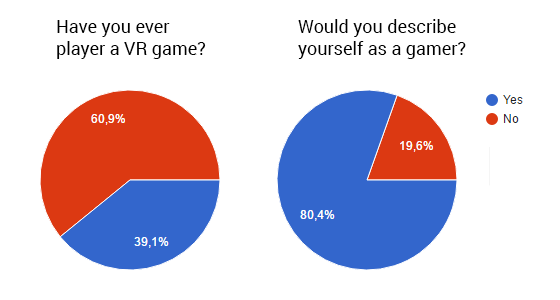
\includegraphics[width=0.90\columnwidth]{./figures/study}
	\caption[study]{Most of the people asked have not tried any VR games yet. Also most of the participants would say they are gamers.}~\label{fig:study}
\end{figure}

\subsection{Motivation In Games}

The staff of \textit{Quantic Foundry}~\cite{online:motivation}  have developed an online survey for categorizing 
gamers and their motivation.%\footnotemark[6]
Users can receive a personalized report on their gaming incentive by completing a survey with about 14 questions on their approach towards games, their different gaming aspects and habits. \newline
Over the course of early 2016 until late august 220 thousand individual people took the test. Among the participants were about 81\% male and 18\% female users. The age ranged from 13 to 77 years and the median was 25 years. Most of the gamers came from North America and the western EU.

The most interesting part is the model that emerged from the data they have got. The categories can be seen in Figure~\ref{fig:gameMotivation}. They have described the categories as follows:

\begin{figure}
	\centering
	\begin{subfigure}[b]{0.49\columnwidth}
		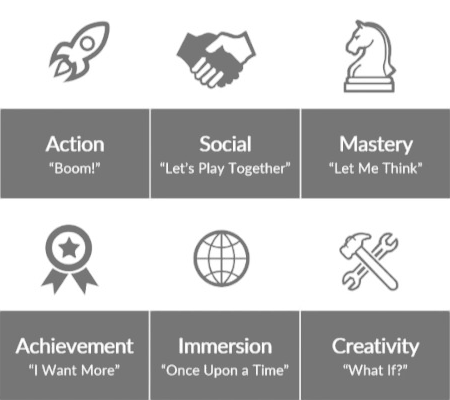
\includegraphics[width=\textwidth]{./figures/motivation}
		\caption[motivation]{Categories of motivation}~\label{fig:gameMotivation}
	\end{subfigure}
	\begin{subfigure}[b]{0.49\columnwidth}
		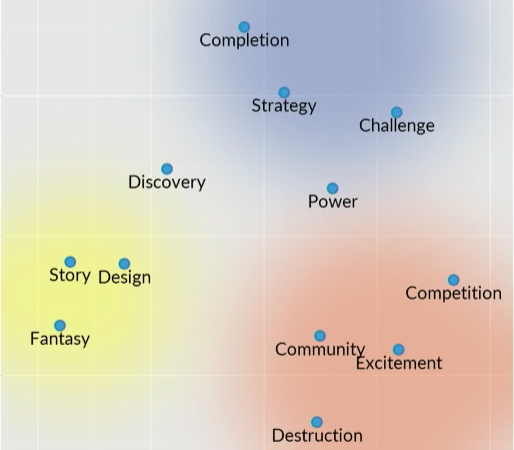
\includegraphics[width=\textwidth]{./figures/clusters}
		\caption[motivation]{Motivational clusters}~\label{fig:motivationClusters}
	\end{subfigure}
	\caption[]{Left: The 6 categories of motivation in games as described by Nick Yee of \textit{Quantic Foundry} in their talk about motivation. | Right: Three motivational clusters that followed from the study of Nick Yee and \textit{Quantic Foundry}. Blue is mastery-achievement cluster, yellow is immersion-creativity cluster and red is action-social cluster. Image source in footnote 3\textcolor{white}{\footnotemark[3]}}
\end{figure}

\footnotetext[3]{"Gamer Motivation Profile Findings - \#GamesUR US Conference 2016" Quantic Foundry Website, March, 25., 2015, accessed November 05., 2016, \url{http://quanticfoundry.com/2016/04/07/gdc-talk/}}

\begin{description}%[align=right,labelwidth=2.5cm]
	\item[Action] \textit{''The appeal of mayhem and chaos and exciting, fast paced game play context.''}~\cite{online:motivation} \newline Action as motivation addresses people who like the thrill and the challenge.
	
	\item[Social] \textit{''Contains both: the challenge and the interesting collaboration and socializing.''}~\cite{online:motivation} \newline The social category describes people who like to socialize, help and/or compete with others.
	
	\item[Mastery] \textit{''Is about long term planning and thinking. Practicing the game to take on the highest difficulty or the enjoyment of strategy.''}~\cite{online:motivation} \newline It mostly appeals to the peoples wish to make complex decisions.
	
	\item[Achievement] \textit{''Different ways of getting points in the context of the game. Credits, points, stars, trophies et cetera. Also, in another way, power. Meaning leveling up or getting the best equipment and gear.''}~\cite{online:motivation} \newline Rouses some peoples collector's passion as well as appeals to people who want to feel powerful.
	
	\item[Immersion] \textit{''Different ways of becoming embedded in the story of the world.''}~\cite{online:motivation} \newline For those people who want to become someone else or want to experienced interesting stories.
	
	\item[Creativity] \textit{''Making the game your own in any kind of way. [...] Uniqueness, customization and discovery.''}~\cite{online:motivation} \newline Mostly describing people who like creativity in games and those who want to customize their experience.

\end{description}

It was found that those gamers that fit into one of the six main categories often prefer similar aspects of a game as that players falling into another of the categories. \newline
From this categorization the next step for them was to analyze their results. They have found that at a high level there are \textit{three} motivational clusters that combine multiple of the categories into sections of similar gaming behaviors. \newline 
These clusters can be seen in Figure~\ref{fig:motivationClusters} and are described as follows:

First there is the \textbf{action-social} cluster, combining the action-packed gameplay with social activities in games. As described before this cluster holds people that like the thrill of the game and want to have action, but it also contains the challenge of the game as well as socializing. It was found that these gamers share some common interests such as \textit{community}, \textit{destruction} and \textit{excitement}. \newline
The second cluster is \textbf{mastery-achievement}, containing players that want to become better. It is standing to reason that these classes are very much correlating in many ways. A multitude of games today offer many ways of collecting items as part of achievements and are also awarding them for collected rare items. A more fine grained description of the people in this category would be to describe them as gamers who like points such as \textit{competition}, \textit{strategy} and \textit{challenge}. \newline
And the last cluster is \textbf{immersion-creativity}. With points like \textit{story}, \textit{fantasy} and \textit{design} it is the most compact in its variance. It does not surprise that immersion correlates with creativity as they are already very similar in many ways. 

They have further found that there are two traits which form kind of like bridges between clusters. \newline
For one that is \textit{discovery}, where the player wants to discover new ways of playing the game as well as discover exciting places inside of the in game world. This can be categorizes both in the \textit{mastery-achievement} and the \textit{immersion-creativity} cluster because it holds aspects from the first as well as the latter.\newline 
The second is indicated as \textit{power}, spanning a bridge between \textit{action-social} and \textit{mastery-achievement}, and appeals to the user to satisfy the urge to master the game and also be in the center of action. 

\divider

In virtual reality not all categories convey easily. While \textit{action}, \textit{immersion} and \textit{creativity} are often already well implemented in todays games missing research on the \textit{social}, \textit{achievement} and \textit{mastery} parts avert a pivotal statement on the subject. \newline
VR games are frequently designed to imply action. Many games use fast-paced gameplay techniques to offer the player thrilling experiences. This arises from the fact that modern HMDs provide not enough comfort to keep playing for very long periods of time. Games therefor have to entertain the user fast and convincing. Also they often require creative problem solving skills of their users and offer great ways of designing or customizing the game.\newline
The immersion is already given by the fact that the user is playing a VR game, so this will not be specified further. 

On the other hand not many approaches have been made to include other real players into the game. With this the social aspect of gaming motivation lacks somewhere behind other categories. A very small fraction of games have a well developed idea of how to include a second player into the game and even less games have a perfect representation of another player in the game, i.e. via avatar. \newline
Gamers can not interact with other people very well while playing VR games, this not only owed to the fact that VR can not yet represent other players well, but also due to the missing presence of items in the real world. An application for real world items is that in games for most social interaction a player can 'trade' items easily. How this problem could be tackled will be discussed in the section \textbf{Further Research Trends}. \newline 
The other two categories have not been developed into VR games a broad as in other games it remains uncertain what will be in the future.

With the previously presented games come different motivational inducements. \newline
In Minecraft, the most frequently played game of the three, motivation will most certainly fall under the creativity point when playing on PC or console without HMDs. Whereas using a VR headset to play it will most likely address immersion at least as much as creativity because the game world and interaction will become more convincing to the user. Hence Minecraft clearly belongs to the \textit{immersion-creativity} cluster both in normal play mode as well as using a HMD.

Keep Talking and Nobody Explodes has already a very immersive approach to playing the game. The view of the player does not differ much from the point of view gained in a the virtual environment, although the user can be even more included when playing with a HMD.

Project CARS recieves more immersiveness as well as a better feeling for the action in the game since it varies much from the gameplay without headset. 

In conclusion, the motivation of all three games gets included or increases in the \textit{immersion} category when using HMDs. The game developers have to implement a well defined method of interaction and a clear way of transferring the feeling inside their games to develop good VR games. 

%\subsection{Input Techniques}
%Because many of the HMD of earlier sections use similar approaches to enable the user to interact with the game this paragraph is only to show some similarities in these. 
%
%Users can often interact with the game via interface devices such as mouse and keyboard, game controller oder steering wheels. For HMD like the \textit{Samsung Gear VR} and the \textit{Daydream View} no generic 
%interfaces are existent. The \textit{Samsung Gear VR} can be extended via gamepad to form a better experience the simplifies interaction with the virtual environments. The \textit{Daydream View} supports a remote control device similar to a gamepad but has less interaction possibilities that other devices.
%
%All the other devices have bundled interaction possibilities to perform even complicated maneuvers in VR. 
%
%From past developments such as the \textit{XBox Kinect} motion tracking was established, using cameras. Nowadays many other approaches are available so that the detection of body parts is not only a visual problem anymore. It was shown that other forms of interaction provide direct feedback to the base system and fit these problems better at these times. To free the users from bulky interfaces the motion tracking with cameras remains a prosperous candidate.
%
%In the following section \textbf{Further Research Trends} some improvements for the interaction with HMD will be discussed.

\subsection{Existing Locomotion Techniques}
\label{sec:exLocomotion}

There are three basic categories of locomotion present at this time in VR: 
\textbf{artificial}, \textbf{natural} and \textbf{cockpit locomotion} as of the Wikipedia article on VR games with Oculus Rift support \cite{wiki:vrOculus}.

The principle described as \textit{artificial locomotion} is the method of 
moving in the virtual environment by triggering interfaces and telling the game 
where the player wants to go. This method is often used because it offers a great 
degree of freedom. But it also has the greatest disadvantage because the users' 
senses provide different signals to the brain and thus holds the greatest 
potential to cause motion sickness.

There are different specific methods of artificial locomotion:
\begin{description}
	\item[Interface movement]By using the provided interface devices the user 
	can steer the virtual representation of himself in different directions. 
	Depending on the game it has up to three dimensions of motion and thus 
	degrees of freedom.
	\item[Point and teleport]The user has to point, using his provided input 
	method on a surface and confirm the selection. The 
	game then moves the camera, the virtual representation of the player, to the 
	location. By using this method the user can move through a world without 
	the need to actual physical change of location. An advantage is that 
	the user can observe at worlds from different points of view.
\end{description}

In \textit{natural locomotion} only the motion and rotation of the users head is used. It requires no movement indicated through an input interface. This interaction method with the game worlds is very static and thus these kind of games do not cause sickness and enable constant mental presence and longer playtimes to the user.

With natural locomotion the user is limited to a local position in the game as well as the virtual environment. But there are also different approaches to making games using this type of locomotion:
\begin{description}
	\item[Interaction with objects]The user can interact with objects right in 
	front and around him. The objects are movable, turnable and sometimes 
	scalable by using the game interfaces.
	\item[Moving the view around the main game object]Inside the game the user can 
	specify from what angle he wants to look at the game objects in focus. 
	Again by using the game interface he can position the camera and with that 
	the position from which he is interacting with the object.
\end{description}

\textit{Cockpit locomotion} in games use a vehicle with a cockpit or stationary interaction space in a movable item to let the player traverse a large environment. Whether this evokes virtual reality sickness varies between persons, the size of the cockpit, and the intensity of the maneuvers that are performed. Generally, users are less likely getting sick if only gentle movements are done.

In cockpit locomotion the movement of the camera is not possible without moving 
the nearby surrounding environment
\begin{description}
	\item[Cockpit]With a near vicinity of objects displaying a cockpit, such as 
	the one of an airplane, a car or comparable vehicles the user can move 
	himself and his surrounding around the virtual game world and with this 
	move from one place to another.
	\item[Stationary Items]Meaning surroundings that are not movable. In this 
	locomotion technique only the orientation of the device the user is using 
	can be changed. This can be adapted to stationary weaponry or other 
	stationary items.
\end{description}

In research are not many approaches to the pros and cons of these different locomotion 
techniques and no clear statement can be given on the best solution. 
Future research trends will be looked at in the following section under 
\textit{Locomotion}.

%\todo{write about locomotion in the 3 games}
